% ─────────────────────────────────────────────────────────────────────────────
% Appendix C: Hypernetwork Architecture Ablations
% ─────────────────────────────────────────────────────────────────────────────

\section*{Appendix C: Hypernetwork Architecture Ablations}
\label{app:hn_ablations}

This appendix documents three architectural ablations that motivated the
hypernetwork configurations used in the main experiments.
Figure~\ref{fig:dh_sweep} establishes the diagnostic capacity level
$d_h = 8$ for the suffocated Split-MNIST regime (Sub-RQ1, Benchmark~1).
Figure~\ref{fig:beta_chunk_sweep} presents the joint sweep over
regularization strength $\beta$ and chunk size $c$ used to select the
operating point for all main hypernetwork experiments.
Figure~\ref{fig:hn_trajectory_c8} traces the per-task evolution of average
accuracy and backward transfer for the Split-CIFAR10 standard hypernetwork
across all five task transitions.

% ── C.1  Hidden-dimension sweep ───────────────────────────────────────────────

\begin{figure}[H]
    \centering
    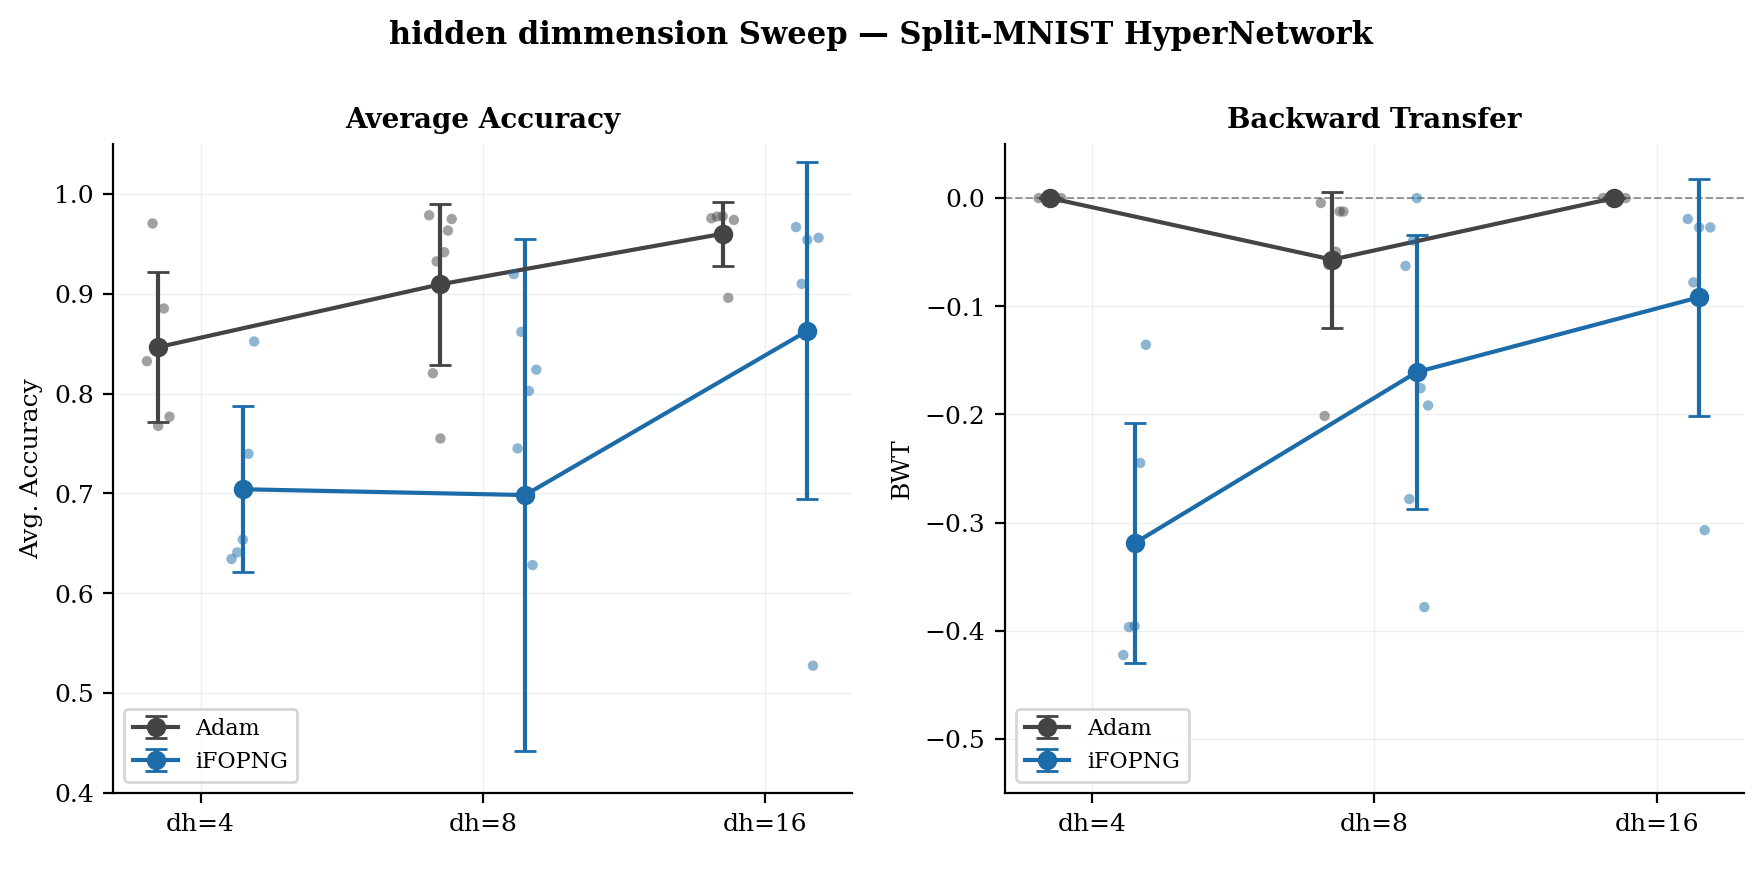
\includegraphics[width=\linewidth]{figures/dh-sweep_7-12-13.png}
    \caption{%
        \textbf{Hidden-dimension sweep --- Split-MNIST SH hypernetwork
        ($d_h \in \{4, 8, 16\}$, 5 tasks, 15 epochs per task,
        \texttt{AdamW} first-task initialisation at $10^{-3}$).}
        Left: average accuracy; right: backward transfer.
        Thick markers show seed means; error bars show $\pm 1$ standard
        deviation; individual seeds are shown as dots.
        Only \texttt{Adam} and \texttt{iFOPNG} are plotted to isolate the
        projection--baseline gap across capacity levels.
        %
        Three capacity levels are compared.
        At $d_h = 4$ (Exp~12), the Adam--iFOPNG gap is $14.0$~pp, but
        individual seed variance for \texttt{iFOPNG} is extreme (range
        $\approx 0.25$), indicating that the bottleneck is too severe for
        reliable projection convergence.
        At $d_h = 8$ (Exp~7), the gap widens to $23.5$~pp and variance
        contracts substantially: seeds cluster in the range $0.63$--$0.92$
        for \texttt{Adam} and $0.63$--$0.75$ for \texttt{iFOPNG}, making
        the failure mode severe and consistently replicable.
        At $d_h = 16$ (Exp~13), projection methods partially recover ---
        the gap narrows to $9.4$~pp --- as the larger gradient budget
        reduces the relative cost of subspace projection.
        %
        The backward transfer panel mirrors this pattern: \texttt{iFOPNG}
        BWT improves monotonically with capacity (${\approx}{-0.32}$ at
        $d_h = 4$, ${\approx}{-0.17}$ at $d_h = 8$,
        ${\approx}{-0.11}$ at $d_h = 16$), while \texttt{Adam} remains
        near zero throughout.
        %
        $d_h = 8$ was retained as the primary diagnostic level: the
        plasticity failure is both severe and consistently replicable,
        whereas $d_h = 4$ yields near-random results in some seeds and
        $d_h = 16$ partially obscures the failure mode.
    }
    \label{fig:dh_sweep}
\end{figure}

% ── C.2  Beta and chunk-size sweep ───────────────────────────────────────────

\begin{figure}[H]
    \centering
    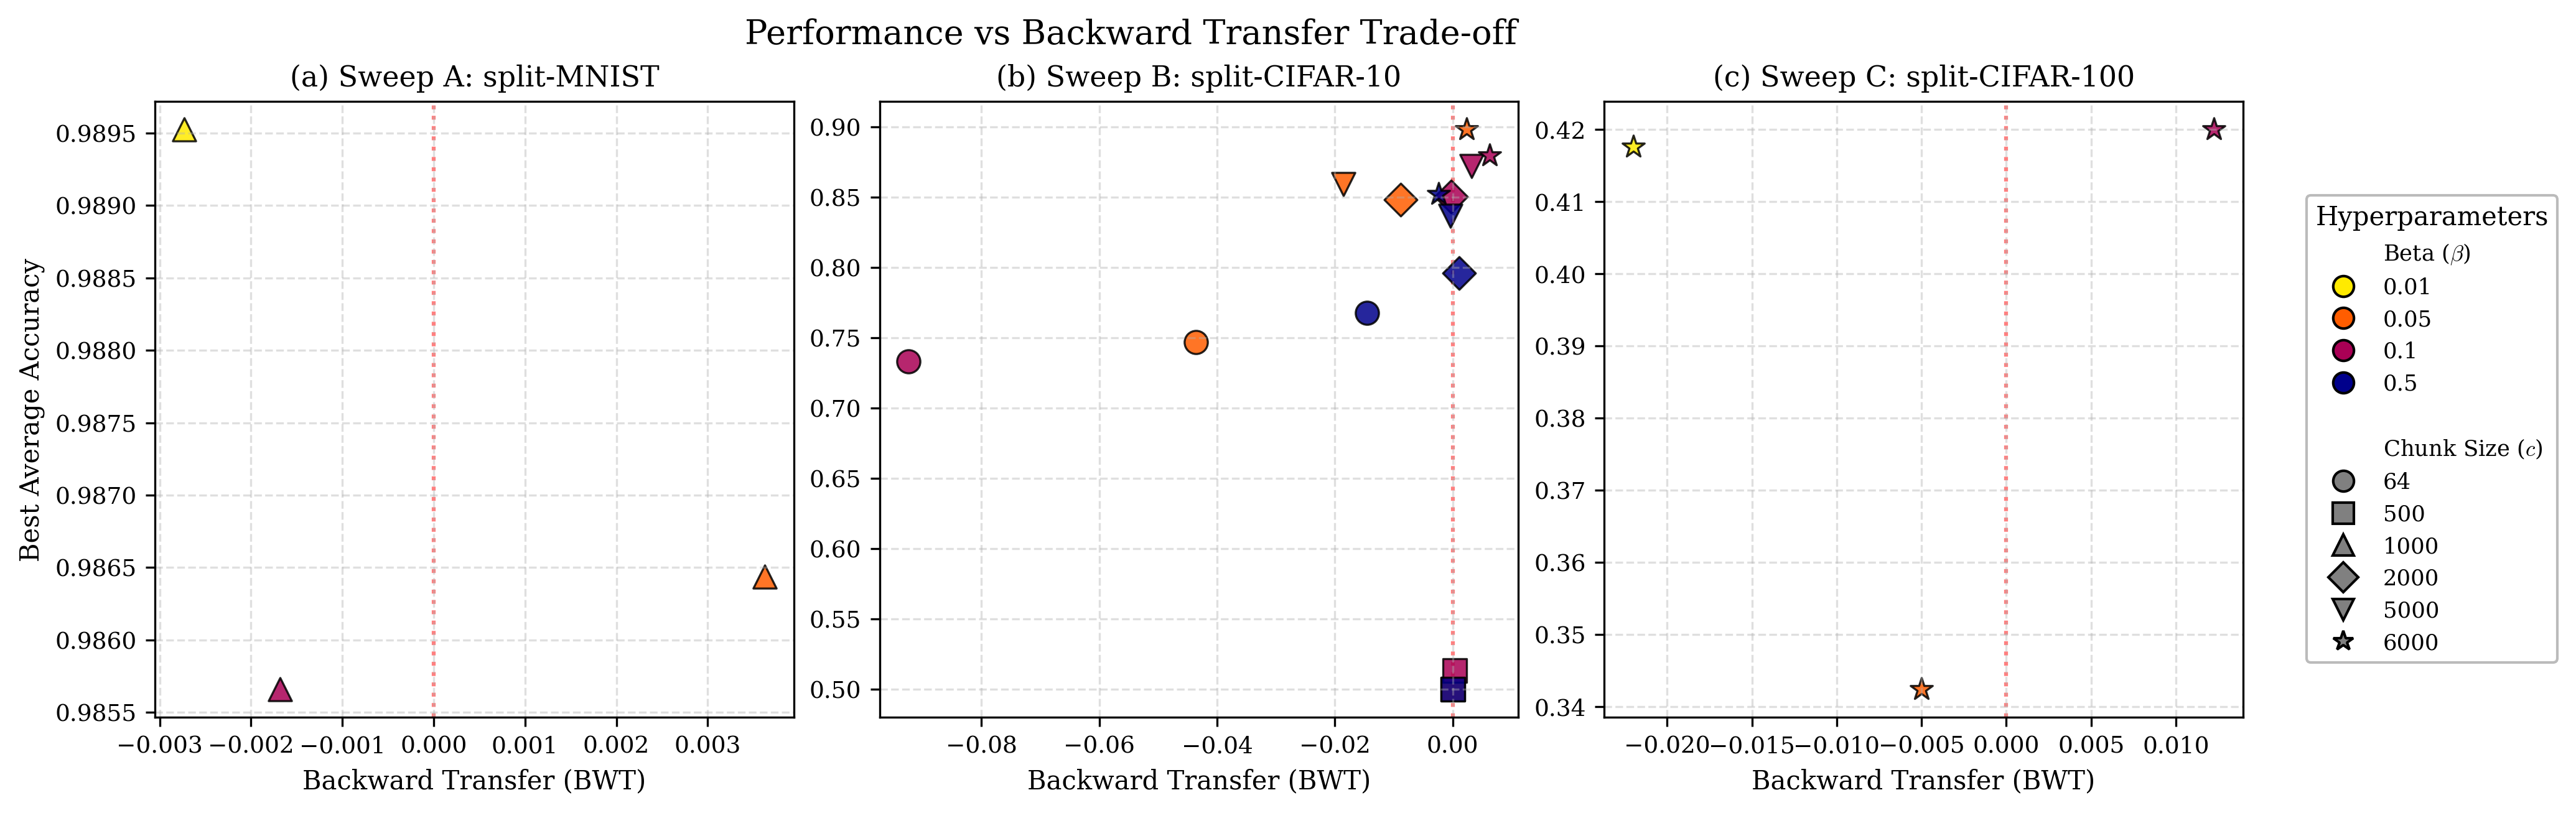
\includegraphics[width=\linewidth]{figures/beta-chunk-sweep_16-17-18.png}
    \caption{%
        \textbf{Beta and chunk-size sweep --- hypernetwork performance
        vs.\ backward transfer trade-off across three benchmarks
        (Exps~16--18).}
        Each panel plots mean average accuracy ($y$-axis) against backward
        transfer ($x$-axis) for all evaluated combinations of regularization
        strength $\beta \in \{0.01, 0.05, 0.1, 0.5\}$ and chunk size
        $c \in \{64, 500, 1000, 2000, 5000, 6000\}$.
        Marker shape encodes chunk size; marker colour encodes $\beta$.
        The vertical red dashed line marks $\mathrm{BWT} = 0$; points
        to its left exhibit net retention, points to its right exhibit net
        forgetting.
        The probe method is \texttt{Adam} with the functional regularizer
        active.
        %
        Split-MNIST (panel a) is insensitive to both hyperparameters: all
        combinations achieve $98.55$--$98.95\%$ accuracy with BWT spanning
        only ${\approx}0.006$, indicating that the task is too simple to
        discriminate architectures.
        %
        Split-CIFAR10 (panel b) shows clear structure. Small chunk sizes
        ($c \in \{64, 500\}$) cluster in the lower-left regardless of
        $\beta$, reaching only $74$--$75\%$ accuracy; larger chunks
        progressively shift the Pareto frontier upward. The combination
        $c = 6000$, $\beta = 0.1$ sits on the efficiency frontier: it
        achieves $87$--$88\%$ average accuracy with small negative BWT,
        providing the best retention--plasticity balance. The combination
        $c = 6000$, $\beta = 0.5$ yields similar accuracy but with
        marginally higher forgetting.
        %
        Split-CIFAR100 (panel c) confirms the selection: $c = 6000$,
        $\beta = 0.5$ achieves the highest accuracy (${\approx}42\%$) but
        at the cost of slightly positive BWT, suggesting the stronger
        regularizer over-constrains plasticity on a 10-task sequence.
        $c = 6000$, $\beta = 0.1$ achieves ${\approx}34\%$ with negative
        BWT and was therefore selected as the operating point for all main
        hypernetwork experiments, providing consistent Pareto-frontier
        performance across both CIFAR benchmarks without the
        positive-BWT artefact observed at higher $\beta$.
    }
    \label{fig:beta_chunk_sweep}
\end{figure}

% ── C.3  Per-task accuracy trajectory — Split-CIFAR10 standard HN ────────────

\begin{figure}[H]
    \centering
    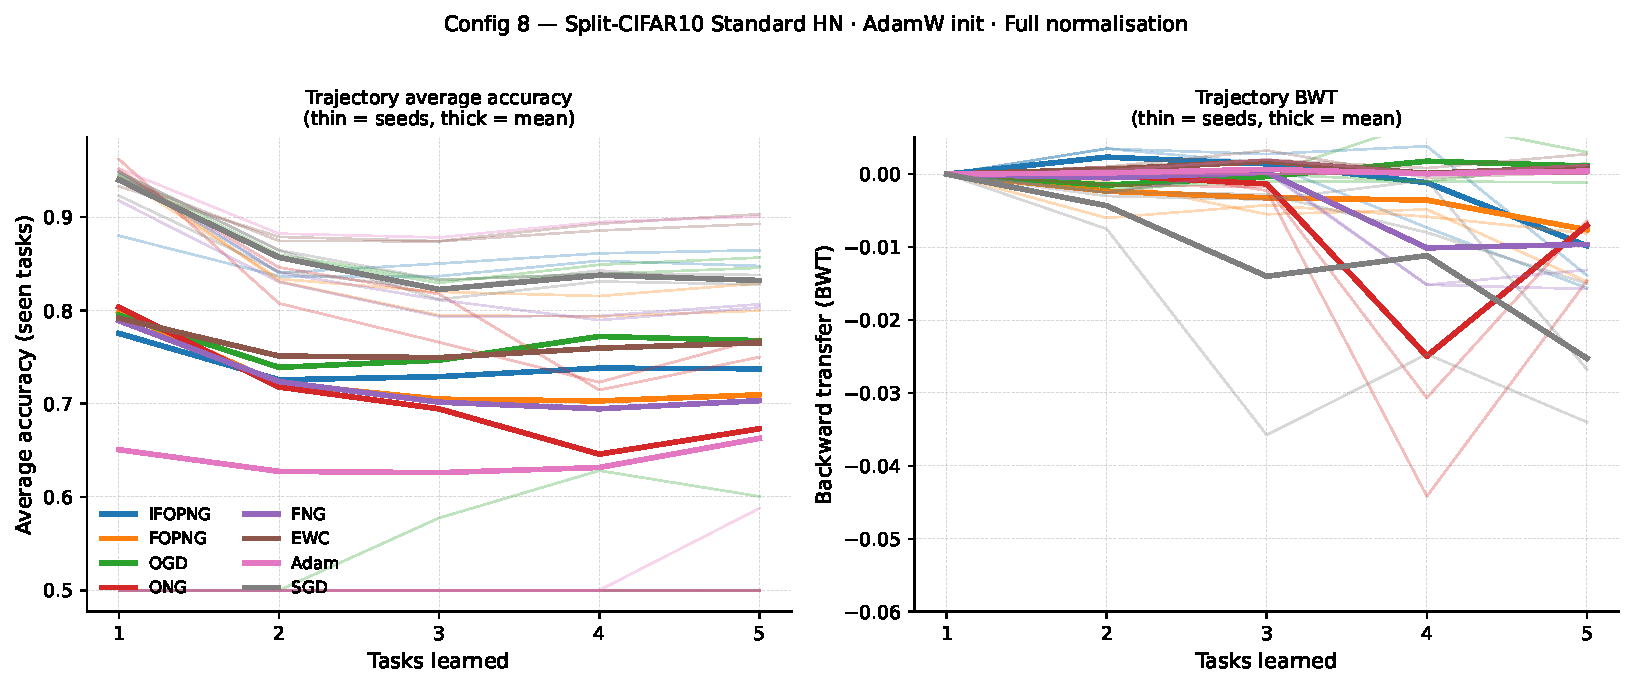
\includegraphics[width=\linewidth]{figures/hypernetwork-heatmaps_8-fig1_trajectory.pdf}
    \caption{%
        \textbf{Per-task learning trajectory --- Split-CIFAR10 standard
        hypernetwork (Config~8, 5 tasks, 50 epochs per task,
        \texttt{AdamW} first-task initialisation, full normalisation).}
        Left: average accuracy over all tasks seen so far, evaluated after
        each task is trained ($x$-axis = number of tasks learned).
        Right: backward transfer over the same sequence.
        Thick lines show the seed mean; thin lines show individual seeds.
        %
        After task~1 all methods achieve high single-task accuracy
        ($0.78$--$0.95$), since no forgetting has yet occurred.
        The stratification that determines the final ordering in the
        main text (Figure~1) is established by task~2 and remains
        largely stable thereafter.
        \texttt{Adam} (pink) maintains the highest trajectory throughout,
        ending at ${\approx}0.84$ and separating from the projection
        cluster at task~2.
        \texttt{SGD} (grey) tracks \texttt{Adam} closely for tasks 1--3
        before diverging slightly downward, reflecting the onset of
        forgetting without momentum.
        \texttt{iFOPNG} (blue), \texttt{EWC} (brown), and \texttt{OGD}
        (green) form a mid-tier cluster between $0.71$ and $0.78$ from
        task~2 onward.
        \texttt{ONG} (red) undergoes a pronounced dip at task~4
        (individual seeds visible in the thin lines), partially recovering
        to ${\approx}0.67$ by task~5; this instability is consistent with
        the high seed variance for \texttt{ONG} reported in the main text.
        %
        The backward transfer panel confirms that the functional
        regularizer suppresses forgetting across all methods: BWT values
        remain within $[{-0.03},\,{+0.01}]$ throughout the full sequence.
        The accuracy gap between \texttt{Adam} and projection methods
        therefore reflects a deficit in forward transfer to newly seen
        tasks rather than differential forgetting of earlier ones --- a
        conclusion consistent with the per-task heatmaps in
        Appendix~D (Figure~\ref{fig:heatmap_c8}).
    }
    \label{fig:hn_trajectory_c8}
\end{figure}